% Incorporates https://gist.github.com/FelipeCortez/10729134

\documentclass{article}

% Package imports
\usepackage{titlesec}
\usepackage{geometry}
\usepackage{fancyhdr}
\usepackage{graphicx}
\usepackage{hyperref} % \url, https://www.overleaf.com/learn/latex/Hyperlinks
\usepackage{outlines} % better itemize
\usepackage{comment}
\usepackage{multirow} % tables
\usepackage{noto-sans} % Google Noto Fonts
\usepackage{hyperref} % Hyperlinks to sectiosn
\usepackage{listings}
\usepackage{lstautogobble} % listings: Fix relative indenting
\usepackage{color} % listings: Code coloring
\usepackage{zi4} % listings: Nice font

\usepackage[british]{datetime2} % load before gitinfo2 to customize
\usepackage[mark=true,grumpy=true]{gitinfo2}

\usepackage{subfiles} % Best loaded last in the preamble

% Redefine \gitMark to customize it
% https://mirror.apps.cam.ac.uk/pub/tex-archive/macros/latex/contrib/gitinfo2/gitinfo2.pdf
\renewcommand{\gitMark}{Branch: \gitBranch\,@\,\gitAbbrevHash{}\,\textbullet{}\,\DTMusedate{gitdate}}

% Use sans font (noto sans) as default font for this document
\renewcommand{\familydefault}{\sfdefault}

% Word style normal margins.
\geometry{a4paper, includeheadfoot, portrait, total={}, top=12.5mm, bottom=12.5mm, left=25.4mm, right=25.4mm}

\graphicspath{ {./images/} }

% Variables
\def\projectname{Inventory Project}

% Override subparagraph with a variant that has no indentation
% https://tex.stackexchange.com/a/392014
\makeatletter
\renewcommand\subparagraph{%
\@startsection{subparagraph}{5}{0pt}%
{3.25ex \@plus 1ex \@minus .2ex}{-1em}%
{\normalfont\normalsize\bfseries}}
\makeatother

\title{\projectname}
\author{James Cahill}
\date{Sepetember 2023}

% Configure fancyHDR page style
% https://tex.stackexchange.com/questions/266911/get-fancyhdr-and-geometry-to-work-nicely
\fancypagestyle{style}{
    \fancyhead{} % clear all header fields
    \fancyhead[HL]{\projectname}
    \fancyhead[HR]{James Cahill}
    \renewcommand{\headrulewidth}{0pt} % Remove header line
}
\pagestyle{style}

% Configure listings colours
\definecolor{bluekeywords}{rgb}{0.13, 0.13, 1}
\definecolor{greencomments}{rgb}{0, 0.5, 0}
\definecolor{redstrings}{rgb}{0.9, 0, 0}
\definecolor{graynumbers}{rgb}{0.5, 0.5, 0.5}

% Configure listings style
\lstset{
    autogobble,
    columns=fullflexible,
    showspaces=false,
    showtabs=false,
    breaklines=true,
    showstringspaces=false,
    breakatwhitespace=true,
    escapeinside={(*@}{@*)},
    commentstyle=\color{greencomments},
    keywordstyle=\color{bluekeywords},
    stringstyle=\color{redstrings},
    numberstyle=\color{graynumbers},
    basicstyle=\ttfamily\footnotesize,
    frame=l,
    framesep=12pt,
    xleftmargin=12pt,
    tabsize=4,
    captionpos=b
}


\begin{document}


\tableofcontents

\pagebreak

\section{Analysis}

% Background
\subsection{Problem Identification}

\subsubsection{Problem Description}
\subfile{sections/analysis/problemIdentification/problemDescription}

\subsubsection{Stakeholders}
\subfile{sections/analysis/problemIdentification/stakeholders}

\subsubsection{Why is it suitable to a computational solution?}

\begin{comment}
why creating this solution is better with the use of technology
eg:
need a way to store large amounts of data; perfect for a database
easy way to add/remove inventory (would be labour intensive otherwise - paper based systems)
can be v. easily done with a gui

identifying key things the solution should have; explain why doing
this computationally is a good idea / is easy

1/2 a page to a page

eg decomposition/abstraction
decomp:
large program; by splitting into smaller sub-programs
can make each one individually and combine at the end
explain how they can be used to achieve the goals/impls
\end{comment}

\subsection{Investigation}

\subsubsection{Preparation for interview}
\subfile{sections/analysis/investigation/prep}

\subsubsection{Interviews}

\begin{comment}
2 or 3

person
question
answer
brief summary
\end{comment}

\subsubsection{Summary of interviews}

\begin{comment}
half a page of key things that were found out from the interviews
should include / should not include / etc.


\end{comment}

\pagebreak

\subsection{Research}


\subsubsection{Existing similar solutions}
\subfile{sections/analysis/research/existing}

\subsubsection{Features to be incorporated into solution}

\begin{comment}
based on research etc
select the features from the research that will be incorporated
and explain what they do
from sortly, steal x feature because y
include things you won't include as well (out of scope), because xyz
\end{comment}

\subsubsection{Limitations of the solution}

\begin{comment}
limitations:

- time

- limited by any software

- money - hosting backend?
- not getting an apple dev account
so won't be a "true" mobile app, more of a website on the home screen.
\end{comment}

\subsubsection{Feedback from stakeholders}

\subsection{Requirements}

\subsubsection{Stakeholder requirements}
\label{sec:stakeholderRequirements}

\pagebreak

\subsubsection{Software and hardware requirements}
\subfile{sections/analysis/requirements/software_hardware}

\pagebreak

\subsubsection{Success requirements}
\subfile{sections/analysis/requirements/success}

\section{Design}

\begin{comment}
design: for each page/screen:

picture of page


brief desc of what the page will do

for each one show the stakeholder requirements or success requirements that will be met when this page/feature is implmented;


then break down each component of the design page.
sentance or two on what it does and why (justify it being there)

\end{comment}

\subsection{User Interface Design}

\subsubsection{Usability Features}

\subsubsection{Feedback from stakeholder}

\subsection{Modular breakdown}

\subsection{Algorithms}

\subsection{Data Dictionary}

\subsection{Inputs and outputs}

\subsection{Validation}

\subsection{Testing}

\subsubsection{Methods}

\subsubsection{Test Plan}

\pagebreak

\section{Implementation}

\subsection{First Iteration | Initial Backend and Database}

\begin{comment}
\subsubsection{Introduction OLD}

\noindent\\ The first thing I decided to work on was user account creation. This would involve using GraphQL to receive data about the new user, generating the user ID, and then placing that data in a database.
After doing some research (should I talk about the different options?) I decided to use the following three libraries for my project:

\begin{outline}
    \1 \textbf{Gin}\\
    Gin is a HTTP framework for Go. This allows me to expose my GraphQL endpoint over HTTP. After conducting some research, I choose to use gin as it is by far the fastest library available at the time of writing.
    It offers performance up to 40 times faster than it's closest alternative, \textit{"Martini"}.
    Gin is a very popular framework, with over 72 thousand stars on GitHub. Using this library benefits me as it has been battle-tested by other users and includes end to end testing, making it more than suitable for my project. (wording isn't great, trying to say it has been tested already)

    \1 \textbf{Gqlgen}\\
    Gqlgen is a Go library designed to make building GraphQL servers easy and hassle-free. It is designed with a schema-first approach, meaning the developer (me) can simply define their API using the standard GraphQL Schema Definition Language. It prioritizes type safety, and has rudimentary validation support built-in. However, I will not be relying on this validation feature, I will create my own validation system that better suits my needs.

    \1 \textbf{GORM} (Go Object Relational Mapping library)\\
    GORM is a fully-features ORM library for Go. (explain what an ORM does)
\end{outline}

\end{comment}

\subsubsection{Introduction}

In this sprint I will work on the backend service.
This service will provide an interface for the frontend to talk to the database via an API (Application Programming Interface).
I am writing the backend in Go, which is a performant, statically typed high level language designed by Google.
Go is frequently used for backend development thanks to it's excellent performance and built in memory safety.
I am also going to use \underline{GraphQL} as the query language used by the frontend to interact with the backend.

\noindent \\ GraphQL is an open-source query and manipulation language designed for use in APIs. The backend will serve as an API which will interface with my database.
I choose to use GraphQL as it is better suited for larger, more complex data sources, and supports querying for multiple different types of data at once, unlike REST. It is also something I was interested in learning more about as I have not designed a system using it before. \\

James: Should this intro be in the design area instead?

TODO: explain what a graphql mutation is (it's a function)

\subsubsection{User account creation}

The first feature I decided to work on was user account creation. This would involve asking the user for an email address, name and password, before validating it and inserting it into the database.
In addition, at a later stage, validation must be performed in order to ensure that:

\begin{itemize}
    \item The user email is not already in use
    \item The generated user ID is unique and not already in use
\end{itemize}

\noindent For this early stage of development, I decided to use an SQLite database to make things easier. I hope that I can easily switch this to PostgreSQL (as specified in my design doc) later on in the development process.

\noindent I have created a GraphQL mutation called \lstinline{createUser}. When it is called, the GraphQL library calls the \lstinline{CreateUser} function, passing any input data from the query.\\ The database connection is available at "\lstinline{r.db}".\\

\noindent My first version of this function was as follows:

\begin{lstlisting}[language=Go]
// CreateUser is the resolver for the createUser field.
func (r *mutationResolver) CreateUser(ctx context.Context, input model.NewUser) (*model.User, error) {
	// Create the user struct
    user := structs.User{FirstName: input.FirstName, LastName: input.LastName, Email: input.Email}
	
    // Generate a user ID
    user.ID = uuid.New()

    // Create the database entry
	r.db.Create(&user)

    // Return the created user data, converting it to a GraphQL model.
	return &model.User{
        ID: user.ID.String(),
        FirstName: user.FirstName,
        LastName: user.LastName,
        Email: user.Email
    }, nil // return nil in the error field
\end{lstlisting}

\noindent \\ The first thing I noticed after implementing this function was that it was tedious to convert back and forth between \lstinline{structs.User} (the database object) and \lstinline{model.User} (the GraphQL object). I decided to merge these into a single object. This was done with the following lines in my GraphQL library's configuration file:

\begin{lstlisting}[language=Python]
models:

[..]

    # Custom models
    Checkout:
      model: github.com/jcxldn/fosscat/backend/structs.Checkout
    Entity:
      model: github.com/jcxldn/fosscat/backend/structs.Entity
    Item:
      model: github.com/jcxldn/fosscat/backend/structs.Item
    User:
      model: github.com/jcxldn/fosscat/backend/structs.User
\end{lstlisting}

This instructs the GraphQL library to use the structs I defined for the database as if they were GraphQL models.

\subparagraph{Unique ID generation}

\noindent \\\\ I decided to use UUIDs (Universal Unique Identifiers) as IDs for all of the objects in my database. (eg. Users, Items) As seen above, I initially choose to simply call \lstinline{uuid.New()} to generate a new random UUID. However, I would soon realise that it would be beneficial to perform \textbf{validation} in order to ensure that the UUIDs were actually unique, ie. that they were not being used by another object of the same type. For example, I wouldn't want two users to have the same User ID.

\noindent \\ I decided to use a \textbf{for loop} to continuously generate UUIDs to be used as a potential User ID. I then perform a database lookup to ensure that the UUID is not already in use.

This can be done with the following code:

\begin{lstlisting}[language=Go]
func (r *mutationResolver) CreateUser(ctx context.Context, input model.NewUser) (*structs.User, error) {

[..]

	isFreeUuid := false
	for !isFreeUuid {
		// Generate a UUID for the user id.
		user.ID = uuid.New()
		// Check that the UUID has not been used already
		// If true, it will break out of this for loop and continue.
		isFreeUuid = util.IsUuidFree[structs.User](r.db, user.ID)
	}

\end{lstlisting}

\noindent In order to achieve this and reduce code duplication across different functions, \\
I created a "IsUuidFree" utility function. Here is the code:

\begin{lstlisting}[language=Go]

func IsUuidFree[T any](db *gorm.DB, id uuid.UUID) bool {
	obj := new(T)
	err := db.Model(obj).Select("id").Where("id == ?", id.String()).First(&obj).Error
	if errors.Is(err, gorm.ErrRecordNotFound) {
		// Record not found, so user id is free
		return true
	} else {
		// Record was returned successfully, therefore the user exists
		return false
	}
}

\end{lstlisting}

JAMES: this initially was different but I changed it to make it simpler. Should I include the old version as well?\\

\noindent This function makes use of \textbf{generics}. As per the Go docs:

\begin{quotation}
    \textit{
        With generics, you can declare and use functions or types that are written to work with any of a set of types provided by calling code.
    }
\end{quotation}

\noindent To simplify, generics mean that I can pass any struct (\textbf{T}) to the function.
For example, if I call the function with:\\

\begin{lstlisting}[language=Go]
    util.IsUuidFree[structs.User](r.db, user.ID)
\end{lstlisting}

\noindent \\Then T is set to the type \lstinline{structs.User}.\\

\noindent \textbf{GORM} (my database library) works by defining a struct to query for which corresponds to a table in the database (in this case the \lstinline{Users} struct corresponds to the \lstinline{users} table). We can then perform SQL actions on this table, such as Select. \\

\noindent Therefore, the GORM db call from above:

\begin{lstlisting}[language=Go]
    db.Model(obj).Select("id").Where("id = ?", id.String()).First(&obj)
\end{lstlisting}

\noindent is the equivalent of:

\begin{lstlisting}[language=SQL]
    SELECT id FROM users WHERE id == ? LIMIT 1 VALUES ("value of id.String()")
\end{lstlisting}

\subparagraph{Testing the user account creation flow}

\noindent \\ Now that I have implemented user account creation, I need to test it to verify that my solution works as expected. I have added a GraphQL query to list all users, which I will use in conjunction with the \lstinline{createUser} mutation.

\noindent \\ I am using a piece of software called \textbf{Altair}, which is an interactive way to make GraphQL queries. I start by creating my GraphQL query which includes the \lstinline{createUser} mutation, making sure to set all required fields:\\

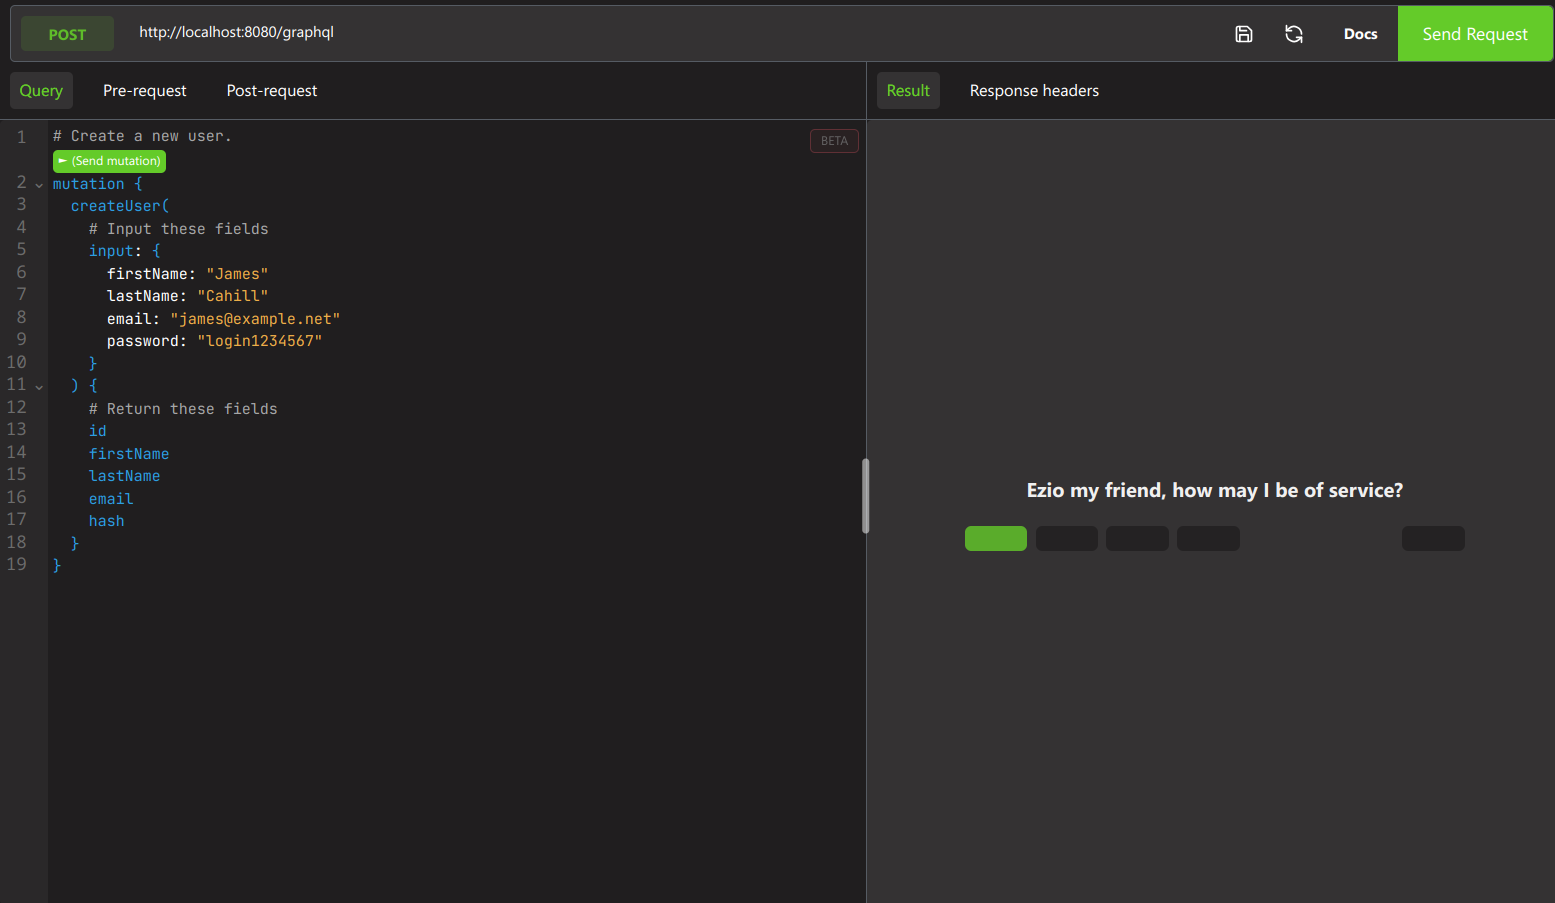
\includegraphics[width=15cm]{implementation/first iteration/createUser altair.png}

\noindent \\ Running the query results in the following response:\\

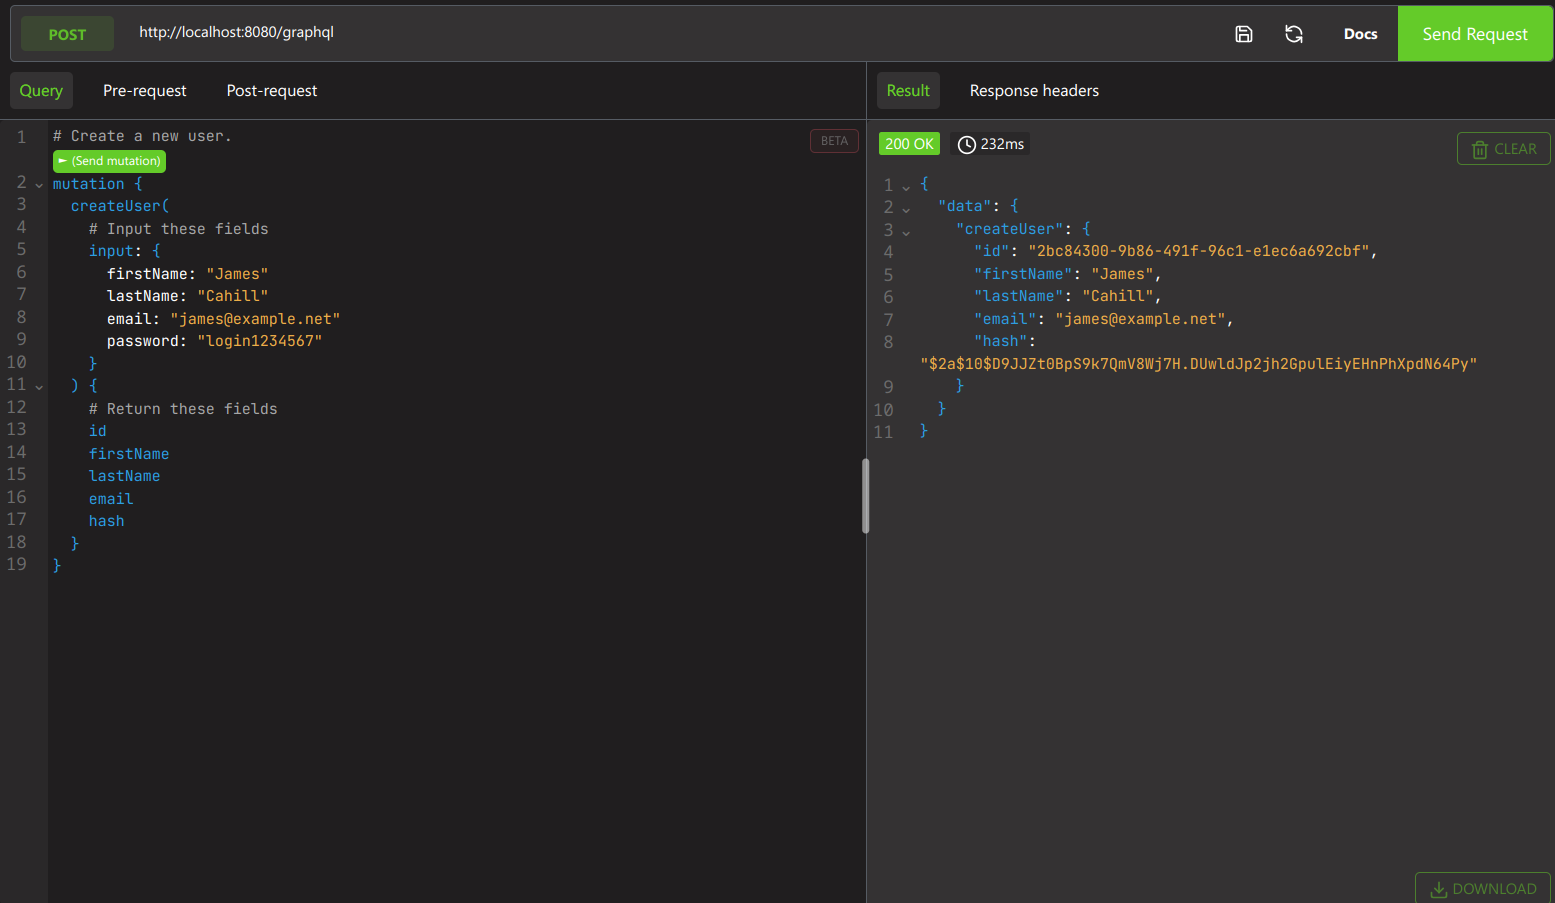
\includegraphics[width=15cm]{implementation/first iteration/createUser altair ran.png}

\noindent \\ Let's check the database for our new user to ensure it was added successfully:\\

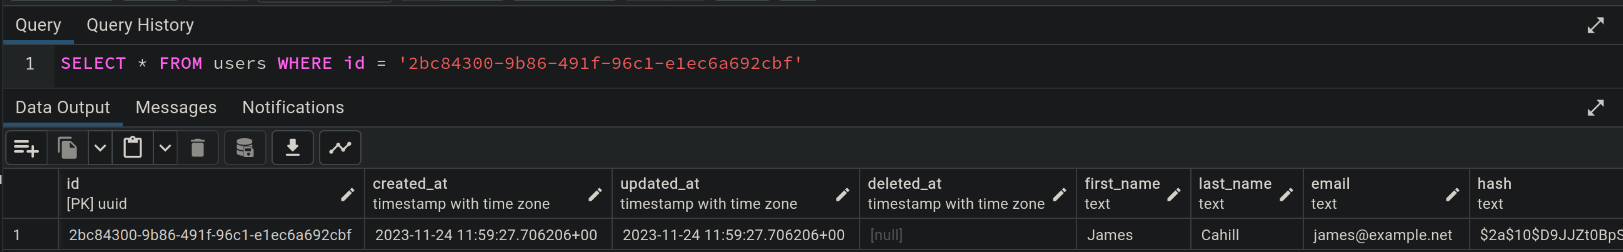
\includegraphics[width=15cm]{implementation/first iteration/createUser query db.png}

\noindent \\ We can see that the user is created successfully, added to the database, and the specified fields (line 12 onwards in the query) are returned to the client.

\subsubsection{Problems encountered when moving to PostgreSQL}

\noindent At this stage, with most of the core functionality implemented, I decided to switch back to PostgreSQL. However, when doing this I encountered two problems:

\subparagraph{Problem 1 - Entity relation errors}

\noindent \\ When creating the database in PostgreSQL, I encountered the following error, displayed in the backend logs.

\begin{lstlisting}[language=SQL]
/backend/database.go:35 ERROR: relation "entities" does not exist (SQLSTATE 42P01)

[17.308ms] [rows:0] CREATE TABLE "checkouts" ("id" text,"created_at" timestamptz,"updated_at" timestamptz,"deleted_at" timestamptz,"take_date" timestamptz,"return_date" timestamptz,PRIMARY KEY ("id"),CONSTRAINT "fk_entities_checkouts" FOREIGN KEY ("id") REFERENCES "entities"("id"))
\end{lstlisting}

\noindent \\ This error could be traced to the following line in my code, where the database is "migrated" by GORM, which means that it attempts to create the necessary tables and columns to match the structs I have defined.

\begin{lstlisting}[language=Go]
    // "Migrate" the schema
	// This will create tables, keys, columns, etc.
	// See https://gorm.io/docs/migration.html
	// Note that we need to pass each struct in our schema.
	db.AutoMigrate(&structs.Checkout{}, &structs.Entity{}, &structs.Item{}, &structs.User{})
\end{lstlisting}

\noindent \\Could do: For example struct A creates this table? show it off?

\noindent \\ This error prevented me from progressing with the backend implementation, as the program would error out during table creation (should I remove this line?)

\noindent \\ After some investigation, I found out that this error occurs when tables that have dependencies on each other are created at the same time (in the same \lstinline{AutoMigrate} call). The fix was to create the dependent table first followed by the table that depended on it, the code for which can be seen below:

\begin{lstlisting}[language=Go]
    // "Migrate" the schema
    // [..]
	db.AutoMigrate(&structs.Checkout{})
	// Item has a dependency on Entity, so do them in the correct order
	// to avoid "relation does not exist" error during table creation.
	db.AutoMigrate(&structs.Entity{})
	db.AutoMigrate(&structs.Item{})
	db.AutoMigrate(&structs.User{})
\end{lstlisting}

\noindent \\ After making this change, I decided to validate and test it before moving on.

\noindent \\ I decided to test this change by first deleting all the database tables and then starting the backend, which should create (or "migrate") all of the tables.

\noindent \\ Firstly I will connect to the database and delete the tables. I have attached the console output and have annotated what I am doing to make it easier to understand.

% Define psql commented language for lstlistings
\lstdefinelanguage{custom_psql_commented}{
    alsoletter={\=,\#,\-},
    keywords={fosscat\=\#, fosscat\-\#},
    morecomment=[l]{//}
}

\begin{lstlisting}[language=custom_psql_commented]
// Run 'psql' to connect to the database
[james@linux cs-coursework]$ psql -h localhost -U fosscat -W
// Enter the password (it is not displayed)
Password: 
psql (15.4, server 16.1 (Debian 16.1-1.pgdg120+1))
WARNING: psql major version 15, server major version 16.
         Some psql features might not work.
Type "help" for help.

// List all tables, we can see that they exist
fosscat=# \dt
          List of relations
 Schema |   Name    | Type  |  Owner  
--------+-----------+-------+---------
 public | checkouts | table | fosscat
 public | entities  | table | fosscat
 public | items     | table | fosscat
 public | users     | table | fosscat
(4 rows)

// Delete the schema containing all of the tables
fosscat=# DROP SCHEMA public CASCADE;
NOTICE:  drop cascades to 4 other objects
DETAIL:  drop cascades to table users
drop cascades to table checkouts
drop cascades to table entities
drop cascades to table items
DROP SCHEMA
// Re-create the schema
fosscat=# CREATE SCHEMA public;
CREATE SCHEMA
// Set default permissions on schema
fosscat=# GRANT ALL ON SCHEMA public TO public;
GRANT
// List all tables, we can see that there aren't any
fosscat=# \dt
Did not find any relations.
// Quit
fosscat-# \q
\end{lstlisting}

\noindent As can be seen above, the database now contains no tables. Next, let's start the backend, where GORM should recreate the database tables. Below is the startup log:

\begin{lstlisting}
[james@linux cs-coursework]$ GIN_MODE=release ./start-backend.sh
2023/12/05 14:23:08 [database] connected. migrating...
2023/12/05 14:23:08 [database] migrated, done.
2023/12/05 14:23:08 [resolver] db not set, setting.
\end{lstlisting}

\noindent You can see that no errors were produced in the console, indicating that all of the necessary tables and columns were created successfully. To check this, let's connect to the database again and list the tables:

\begin{lstlisting}[language=custom_psql_commented]
// Run 'psql' to connect to the database
[james@linux cs-coursework]$ psql -h localhost -U fosscat -W
// Enter the password (it is not displayed)
Password: 
psql (15.4, server 16.1 (Debian 16.1-1.pgdg120+1))
WARNING: psql major version 15, server major version 16.
         Some psql features might not work.
Type "help" for help.

// List all tables, we can see that they exist
fosscat=# \dt
          List of relations
 Schema |   Name    | Type  |  Owner  
--------+-----------+-------+---------
 public | checkouts | table | fosscat
 public | entities  | table | fosscat
 public | items     | table | fosscat
 public | users     | table | fosscat
(4 rows)

// Quit
fosscat=# \q
\end{lstlisting}

\noindent We can see that the tables were created successfully.

\subparagraph{Problem 2 - Operator does not exist}

\noindent \\ However, when attempting to create a new user in the database I encountered another error:

\begin{lstlisting}[language=SQL]
./backend/util/user.go:14 ERROR: operator does not exist: text == unknown (SQLSTATE 42883)

[0.369ms] [rows:0] SELECT "id" FROM "users" WHERE id == '8596a222-930e-42f0-841e-9d95993668a4' AND "users"."deleted_at" IS NULL ORDER BY "users"."id" LIMIT 1
\end{lstlisting}

\noindent \\ This error states that it cannot compare \lstinline{id} with the given UUID (\lstinline{'8596a222-930e-42f0-841e-9d95993668a4'}) because the operator \lstinline{==} does not exist.
This error points to my \lstinline{IsUuidFree} function, which I talked about in the \textbf{User account creation} section of this iteration.

\noindent \\ After some research, I found that the error occurs because the operator \lstinline{==} does not exist in PostgreSQL. \lstinline{==} is commonly used in programming languages to perform a deep comparison of two objects, and I assumed that the same would be true for PostgreSQL.
Interestingly, the issue did not manifest itself until after the switch to PostgreSQL, meaning that SQLite handles \lstinline{==} as I expected.
The fix was simple; Change \lstinline{'=='} to \lstinline{'='}.

\noindent \\ This meant that the line

\begin{lstlisting}[language=Go]
    err := db.Model(obj).Select("id").Where("id == ?", id.String()).First(&obj).Error
\end{lstlisting}

\noindent became

\begin{lstlisting}[language=Go]
    err := db.Model(obj).Select("id").Where("id = ?", id.String()).First(&obj).Error
\end{lstlisting}

\begin{comment}
POLISH END
\end{comment}

\subparagraph{Problem 3 - "... violates foreign key constraint"}

\noindent \\ When trying to create a new user, the following error message would appear:

\begin{lstlisting}[language=SQL]
/backend/graph/resolver/mutation.go:90 ERROR: insert or update on table "users" violates foreign key constraint "fk_checkouts_user" (SQLSTATE 23503)
[2.691ms] [rows:0] INSERT INTO "users" ("id", "created_at", "updated_at", "deleted_at", "first_name", "last_name", "email", "hash") VALUES [..]
\end{lstlisting}

\noindent This error occurred when trying to create a user. Upon reading into it the error occurred because of how I defined my foreign keys for GORM. For example, I had the following struct definition for \lstinline{Checkout}:

\begin{lstlisting}[language=Go]
type Checkout struct {
	gorm.Model
	ID         uuid.UUID
	User       User `gorm:"foreignKey:ID"`
	TakeDate   time.Time
	ReturnDate time.Time
}
\end{lstlisting}

\noindent Upon reading the GORM documentation, I realised this should actually be:

\begin{lstlisting}[language=Go]
// Checkout belongs to a User, User.ID (UserID) is the foreign key
type Checkout struct {
    gorm.Model
    ID         uuid.UUID
    User       User
    UserID     uuid.UUID
    TakeDate   time.Time
    ReturnDate time.Time
}
\end{lstlisting}

\noindent After applying this change, the program worked as expected. I tested everything by attempting to create a new user in Altair:\\

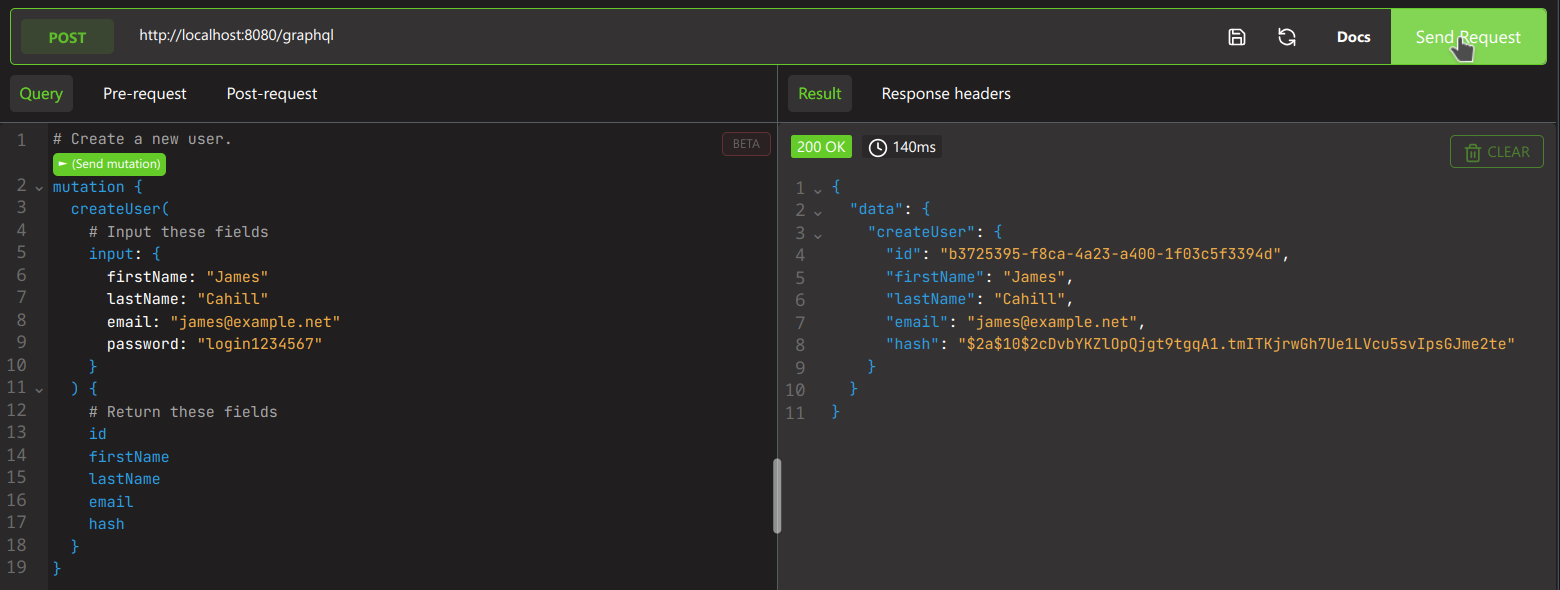
\includegraphics[width=15cm]{implementation/first iteration/postgreproblems altair working.png}

\noindent \\ This query returned successfully and the user was created without any errors.

\subsubsection{Adding foreign keys for lists}

\subsubsection{Issues with nested queries (queries using multiple tables)}

\subsubsection{Adding the remaining queries}

CreateCheckout validation

\subsubsection{Testing}

\paragraph{Test Plan}

\paragraph{Test Results}

\paragraph{Errors encountered during testing}

\subparagraph{Summary}

\subparagraph{Fixing error XYZ}

\subsubsection{Evaluation}

\noindent In this iteration, I have successfully written code that can create a database, create the necessary tables to store data, and exposes functions to create and store data in the database.

\noindent \\ Using GraphQL, user accounts can be created, where a unused unique identifier is found and used, as well as the creation of a salted password hash to securely store the user's password. In addition, checkouts, entities and items can be created each with their unique identifiers. Where necessary, such as with an checkout, we can use relationships to tie the checkout to a specified user object residing in the database.

\noindent \\ The next iteration will focus on adding security to the backend. For example, I will need to add authenticated routes, where users can only view the contents of the route if they are logged in, as it will contain sensitive data.

\pagebreak

\section{Testing}

\section{Evaluation}

\end{document}